\documentclass{article}\usepackage[]{graphicx}\usepackage[]{color}
%% maxwidth is the original width if it is less than linewidth
%% otherwise use linewidth (to make sure the graphics do not exceed the margin)
\makeatletter
\def\maxwidth{ %
  \ifdim\Gin@nat@width>\linewidth
    \linewidth
  \else
    \Gin@nat@width
  \fi
}
\makeatother

\definecolor{fgcolor}{rgb}{0.345, 0.345, 0.345}
\newcommand{\hlnum}[1]{\textcolor[rgb]{0.686,0.059,0.569}{#1}}%
\newcommand{\hlstr}[1]{\textcolor[rgb]{0.192,0.494,0.8}{#1}}%
\newcommand{\hlcom}[1]{\textcolor[rgb]{0.678,0.584,0.686}{\textit{#1}}}%
\newcommand{\hlopt}[1]{\textcolor[rgb]{0,0,0}{#1}}%
\newcommand{\hlstd}[1]{\textcolor[rgb]{0.345,0.345,0.345}{#1}}%
\newcommand{\hlkwa}[1]{\textcolor[rgb]{0.161,0.373,0.58}{\textbf{#1}}}%
\newcommand{\hlkwb}[1]{\textcolor[rgb]{0.69,0.353,0.396}{#1}}%
\newcommand{\hlkwc}[1]{\textcolor[rgb]{0.333,0.667,0.333}{#1}}%
\newcommand{\hlkwd}[1]{\textcolor[rgb]{0.737,0.353,0.396}{\textbf{#1}}}%

\usepackage{framed}
\makeatletter
\newenvironment{kframe}{%
 \def\at@end@of@kframe{}%
 \ifinner\ifhmode%
  \def\at@end@of@kframe{\end{minipage}}%
  \begin{minipage}{\columnwidth}%
 \fi\fi%
 \def\FrameCommand##1{\hskip\@totalleftmargin \hskip-\fboxsep
 \colorbox{shadecolor}{##1}\hskip-\fboxsep
     % There is no \\@totalrightmargin, so:
     \hskip-\linewidth \hskip-\@totalleftmargin \hskip\columnwidth}%
 \MakeFramed {\advance\hsize-\width
   \@totalleftmargin\z@ \linewidth\hsize
   \@setminipage}}%
 {\par\unskip\endMakeFramed%
 \at@end@of@kframe}
\makeatother

\definecolor{shadecolor}{rgb}{.97, .97, .97}
\definecolor{messagecolor}{rgb}{0, 0, 0}
\definecolor{warningcolor}{rgb}{1, 0, 1}
\definecolor{errorcolor}{rgb}{1, 0, 0}
\newenvironment{knitrout}{}{} % an empty environment to be redefined in TeX

\usepackage{alltt}

\title{Problem Set 2}
\author{Tony Lashley}
\date{April 13, 2015}

\usepackage{natbib}
\usepackage{graphicx}
\graphicspath{{/Users/Tony/Pictures/}}
\IfFileExists{upquote.sty}{\usepackage{upquote}}{}
\begin{document}
\maketitle

\section{Machinery for the Schelling Model}
\subsection{Write a function that calculates distances between coordinate points}
\begin{knitrout}
\definecolor{shadecolor}{rgb}{0.969, 0.969, 0.969}\color{fgcolor}\begin{kframe}
\begin{alltt}
\hlstd{an_individual} \hlkwb{<-} \hlkwd{c}\hlstd{(}\hlnum{0}\hlstd{,}\hlnum{0}\hlstd{)}

\hlstd{neighbors} \hlkwb{=} \hlkwd{matrix}\hlstd{(}\hlnum{1}\hlopt{:}\hlnum{8}\hlstd{,} \hlkwc{ncol} \hlstd{=} \hlnum{2}\hlstd{,} \hlkwc{byrow} \hlstd{= T)}
\hlkwd{print}\hlstd{(neighbors)}
\end{alltt}
\begin{verbatim}
##      [,1] [,2]
## [1,]    1    2
## [2,]    3    4
## [3,]    5    6
## [4,]    7    8
\end{verbatim}
\begin{alltt}
\hlkwd{colnames}\hlstd{(neighbors)} \hlkwb{<-} \hlkwd{c}\hlstd{(}\hlstr{"X"}\hlstd{,}\hlstr{"Y"}\hlstd{)}
\hlstd{dstances} \hlkwb{=} \hlkwd{matrix}\hlstd{(}\hlkwc{ncol} \hlstd{=} \hlnum{3}\hlstd{,} \hlkwc{byrow} \hlstd{= T)}
\hlkwd{colnames}\hlstd{(dstances)} \hlkwb{<-} \hlkwd{c}\hlstd{(}\hlstr{"X"}\hlstd{,}\hlstr{"Y"}\hlstd{,} \hlstr{"Pythgorean"}\hlstd{)}

\hlstd{f1} \hlkwb{<-} \hlkwa{function}\hlstd{(}\hlkwc{an_individual}\hlstd{,} \hlkwc{neighbors}\hlstd{)\{}

  \hlkwa{for} \hlstd{(i} \hlkwa{in} \hlnum{1}\hlopt{:}\hlkwd{nrow}\hlstd{(neighbors))\{}

    \hlstd{neighbor_longitude} \hlkwb{=} \hlstd{neighbors[i,}\hlnum{1}\hlstd{]}
    \hlcom{## Find your neighbor's longitude}
    \hlstd{neighbor_latitude} \hlkwb{=}  \hlstd{neighbors[i,}\hlnum{2}\hlstd{]}
    \hlcom{## Find your neighbor's latitude}
    \hlstd{individual_longitude} \hlkwb{=} \hlstd{an_individual[}\hlnum{1}\hlstd{]}
    \hlcom{## Find your own longitude}
    \hlstd{individual_latitude} \hlkwb{=}  \hlstd{an_individual[}\hlnum{2}\hlstd{]}
    \hlcom{## Find your own latitude}

    \hlstd{lftrghtdstance} \hlkwb{=} \hlkwd{abs}\hlstd{(neighbor_longitude} \hlopt{-} \hlstd{individual_longitude)}
    \hlcom{## Find east/west distance between indiv. and neighbor}
    \hlstd{updowndstance} \hlkwb{=} \hlkwd{abs}\hlstd{(neighbor_latitude} \hlopt{-} \hlstd{individual_latitude)}
    \hlcom{## Find north/south distance between indiv. and neighbor}
    \hlstd{pyth} \hlkwb{=} \hlkwd{sqrt}\hlstd{(((lftrghtdstance)}\hlopt{^}\hlnum{2}\hlstd{)} \hlopt{+} \hlstd{((updowndstance)}\hlopt{^}\hlnum{2}\hlstd{))}
    \hlcom{## Find Euclidian distance}
    \hlstd{currentdistance} \hlkwb{=} \hlkwd{c}\hlstd{(lftrghtdstance,updowndstance,pyth)}
    \hlcom{## Make vector with Manhattan and Euclidian distances}


    \hlstd{dstances} \hlkwb{<-} \hlkwd{rbind}\hlstd{(dstances, currentdistance)}
    \hlcom{## Add vector as row in matrix of distances}
  \hlstd{\}}

  \hlkwd{return}\hlstd{(dstances)}
\hlstd{\}}

\hlkwd{f1}\hlstd{(an_individual, neighbors)}
\end{alltt}
\begin{verbatim}
##                  X  Y Pythgorean
##                 NA NA         NA
## currentdistance  1  2   2.236068
## currentdistance  3  4   5.000000
## currentdistance  5  6   7.810250
## currentdistance  7  8  10.630146
\end{verbatim}
\end{kframe}
\end{knitrout}

\subsection{Write a function that simulates Schelling's Segregation model}
\begin{knitrout}
\definecolor{shadecolor}{rgb}{0.969, 0.969, 0.969}\color{fgcolor}\begin{kframe}
\begin{alltt}
\hlkwd{library}\hlstd{(RANN)}
\hlkwd{library}\hlstd{(FNN)}
\hlkwd{library}\hlstd{(ggplot2)}
\hlkwd{library}\hlstd{(reshape2)}

\hlkwd{library}\hlstd{(foreach)}
\hlkwd{library}\hlstd{(doParallel)}
\end{alltt}


{\ttfamily\noindent\itshape\color{messagecolor}{\#\# Loading required package: iterators\\\#\# Loading required package: parallel}}\begin{alltt}
\hlkwd{library}\hlstd{(parallel)}

\hlkwd{require}\hlstd{(foreach)}
\hlkwd{require}\hlstd{(doParallel)}
\hlkwd{require}\hlstd{(parallel)}
\hlkwd{require}\hlstd{(ggplot2)}

\hlstd{numCores} \hlkwb{<-} \hlkwd{detectCores}\hlstd{()}
\hlstd{cl} \hlkwb{<-} \hlkwd{makeCluster}\hlstd{(numCores)}
\hlkwd{registerDoParallel}\hlstd{(cl)}

\hlstd{testv} \hlkwb{=} \hlnum{100}

\hlstd{testRacialPreferenceTable} \hlkwb{<-} \hlkwd{matrix}\hlstd{(}\hlnum{1}\hlopt{:}\hlnum{15}\hlstd{,} \hlkwc{ncol} \hlstd{=} \hlnum{5}\hlstd{,} \hlkwc{nrow} \hlstd{=} \hlnum{3}\hlstd{)}
\hlstd{testRacialPreferenceTable[}\hlnum{1}\hlstd{,]} \hlkwb{<-} \hlkwd{c}\hlstd{(}\hlstr{"R"}\hlstd{,}\hlnum{1}\hlstd{,} \hlnum{50}\hlstd{,} \hlnum{5}\hlstd{,} \hlnum{2}\hlstd{)}
\hlstd{testRacialPreferenceTable[}\hlnum{2}\hlstd{,]} \hlkwb{<-} \hlkwd{c}\hlstd{(}\hlstr{"G"}\hlstd{,} \hlnum{0}\hlstd{,} \hlnum{50}\hlstd{,} \hlnum{5}\hlstd{,} \hlnum{2}\hlstd{)}
\hlstd{testRacialPreferenceTable[}\hlnum{3}\hlstd{,]} \hlkwb{<-} \hlkwd{c}\hlstd{(}\hlstr{"B"}\hlstd{,} \hlopt{-}\hlnum{1}\hlstd{,} \hlnum{50}\hlstd{,} \hlnum{5}\hlstd{,} \hlnum{2}\hlstd{)}
\hlkwd{colnames}\hlstd{(testRacialPreferenceTable)} \hlkwb{<-} \hlkwd{c}\hlstd{(}\hlstr{"Color"}\hlstd{,} \hlstr{"Value"}\hlstd{,} \hlstr{"Pop."}\hlstd{,} \hlstr{"Test Pool Size"}\hlstd{,} \hlstr{"Racial Threshold"}\hlstd{)}
\hlkwd{print}\hlstd{(testRacialPreferenceTable)}
\end{alltt}
\begin{verbatim}
##      Color Value Pop. Test Pool Size Racial Threshold
## [1,] "R"   "1"   "50" "5"            "2"             
## [2,] "G"   "0"   "50" "5"            "2"             
## [3,] "B"   "-1"  "50" "5"            "2"
\end{verbatim}
\begin{alltt}
\hlstd{nR} \hlkwb{<-} \hlkwd{as.numeric}\hlstd{(testRacialPreferenceTable[}\hlnum{1}\hlstd{,}\hlstr{"Pop."}\hlstd{])}
\hlstd{nG} \hlkwb{<-} \hlkwd{as.numeric}\hlstd{(testRacialPreferenceTable[}\hlnum{2}\hlstd{,}\hlstr{"Pop."}\hlstd{])}
\hlstd{nB} \hlkwb{<-} \hlkwd{as.numeric}\hlstd{(testRacialPreferenceTable[}\hlnum{3}\hlstd{,}\hlstr{"Pop."}\hlstd{])}

\hlstd{n} \hlkwb{<-} \hlkwd{sum}\hlstd{(nR} \hlopt{+} \hlstd{nG} \hlopt{+} \hlstd{nB)}
\hlcom{## Find total population from summing each racial population}

\hlstd{inputs} \hlkwb{<-} \hlstd{testRacialPreferenceTable}

\hlstd{stop.val} \hlkwb{<-} \hlnum{.95}
\hlstd{happy_counter} \hlkwb{<-} \hlnum{0}


\hlstd{Schelling} \hlkwb{<-} \hlkwa{function}\hlstd{(}\hlkwc{racialPreferenceTable} \hlstd{= testRacialPreferenceTable,} \hlkwc{cyclemax} \hlstd{= testv)\{}
  \hlkwd{set.seed}\hlstd{(}\hlnum{20016}\hlstd{)}
  \hlkwd{library}\hlstd{(ggplot2)}
  \hlstd{LocationTable} \hlkwb{<-} \hlkwd{matrix}\hlstd{(}\hlkwc{ncol} \hlstd{=} \hlnum{3}\hlstd{)}
  \hlcom{## Initalizing table for initial neighborhood coordinates}

  \hlkwa{for} \hlstd{(i} \hlkwa{in} \hlnum{1}\hlopt{:}\hlstd{nR)\{}
    \hlstd{x} \hlkwb{<-} \hlkwd{runif}\hlstd{(}\hlnum{1}\hlstd{,} \hlkwc{min}\hlstd{=}\hlnum{0}\hlstd{,} \hlkwc{max}\hlstd{=}\hlnum{1}\hlstd{)}
    \hlcom{## Generate random X coordinate between 0 and 1 for point}
    \hlstd{y} \hlkwb{<-} \hlkwd{runif}\hlstd{(}\hlnum{1}\hlstd{,} \hlkwc{min}\hlstd{=}\hlnum{0}\hlstd{,} \hlkwc{max}\hlstd{=}\hlnum{1}\hlstd{)}
    \hlcom{## Generate random Y coordinate between 0 and 1 for point}
    \hlstd{R} \hlkwb{=} \hlkwd{c}\hlstd{(}\hlnum{1}\hlstd{,x,y)}
    \hlcom{## Create vector with point coordinates, labeling point as red}
    \hlstd{LocationTable} \hlkwb{<-} \hlkwd{rbind}\hlstd{(LocationTable, R)}
    \hlcom{## Add red point to table of all neighborhood coordinates}
  \hlstd{\}}

  \hlkwa{for} \hlstd{(i} \hlkwa{in} \hlnum{1}\hlopt{:}\hlstd{nG)\{}
    \hlstd{x} \hlkwb{<-} \hlkwd{runif}\hlstd{(}\hlnum{1}\hlstd{,} \hlkwc{min}\hlstd{=}\hlnum{0}\hlstd{,} \hlkwc{max}\hlstd{=}\hlnum{1}\hlstd{)}
    \hlstd{y} \hlkwb{<-} \hlkwd{runif}\hlstd{(}\hlnum{1}\hlstd{,} \hlkwc{min}\hlstd{=}\hlnum{0}\hlstd{,} \hlkwc{max}\hlstd{=}\hlnum{1}\hlstd{)}

    \hlstd{G} \hlkwb{=} \hlkwd{c}\hlstd{(}\hlnum{0}\hlstd{,x,y)}

    \hlstd{LocationTable} \hlkwb{<-} \hlkwd{rbind}\hlstd{(LocationTable, G)}
  \hlstd{\}}

  \hlkwa{for} \hlstd{(i} \hlkwa{in} \hlnum{1}\hlopt{:}\hlstd{nB)\{}
    \hlstd{x} \hlkwb{<-} \hlkwd{runif}\hlstd{(}\hlnum{1}\hlstd{,} \hlkwc{min}\hlstd{=}\hlnum{0}\hlstd{,} \hlkwc{max}\hlstd{=}\hlnum{1}\hlstd{)}
    \hlstd{y} \hlkwb{<-} \hlkwd{runif}\hlstd{(}\hlnum{1}\hlstd{,} \hlkwc{min}\hlstd{=}\hlnum{0}\hlstd{,} \hlkwc{max}\hlstd{=}\hlnum{1}\hlstd{)}
    \hlstd{B} \hlkwb{=} \hlkwd{c}\hlstd{(}\hlopt{-}\hlnum{1}\hlstd{,x,y)}

    \hlstd{LocationTable} \hlkwb{<-} \hlkwd{rbind}\hlstd{(LocationTable, B)}
  \hlstd{\}}

  \hlstd{LocationTable} \hlkwb{<-} \hlstd{LocationTable[}\hlopt{-}\hlnum{1}\hlstd{,]}
  \hlstd{Count} \hlkwb{<-} \hlkwd{c}\hlstd{(}\hlnum{1}\hlopt{:}\hlkwd{nrow}\hlstd{(LocationTable))}
  \hlcom{## Create column counting number of points or people}

  \hlstd{Happy} \hlkwb{<-} \hlkwd{c}\hlstd{(}\hlkwd{rep}\hlstd{(}\hlnum{0}\hlstd{,} \hlkwd{nrow}\hlstd{(LocationTable)))}
  \hlcom{## Create column to keep track of if person is happy}

  \hlstd{Testpool} \hlkwb{<-} \hlkwd{c}\hlstd{(}\hlkwd{rep}\hlstd{(}\hlnum{0}\hlstd{,} \hlkwd{nrow}\hlstd{(LocationTable)))}
  \hlcom{## Create column for indvidual's testpool}

  \hlstd{Threshold} \hlkwb{<-} \hlkwd{c}\hlstd{(}\hlkwd{rep}\hlstd{(}\hlnum{0}\hlstd{,} \hlkwd{nrow}\hlstd{(LocationTable)))}
  \hlcom{## Create column for indvidual's threshold}

  \hlstd{LocationTable} \hlkwb{<-} \hlkwd{cbind}\hlstd{(Count, LocationTable, Happy, Testpool, Threshold)}
  \hlcom{## Add columns to Location Table}


  \hlstd{p} \hlkwb{<-} \hlkwd{qplot}\hlstd{(}\hlkwc{x} \hlstd{= LocationTable[,}\hlnum{3}\hlstd{],} \hlkwc{y} \hlstd{= LocationTable [,}\hlnum{4}\hlstd{],} \hlkwc{col} \hlstd{=} \hlkwd{ifelse}\hlstd{(LocationTable[,}\hlnum{2}\hlstd{]} \hlopt{< -}\hlnum{0.5}\hlstd{,} \hlstr{"red"}\hlstd{,} \hlkwd{ifelse}\hlstd{(LocationTable[,}\hlnum{2}\hlstd{]} \hlopt{<} \hlnum{0.5}\hlstd{,} \hlstr{"green"}\hlstd{,} \hlstr{"blue"}\hlstd{)))} \hlopt{+} \hlkwd{theme}\hlstd{(}\hlkwc{legend.position} \hlstd{=} \hlstr{"none"}\hlstd{)}

  \hlkwd{print}\hlstd{(p)}

  \hlstd{testpoolR} \hlkwb{<-} \hlkwd{as.numeric}\hlstd{(racialPreferenceTable[}\hlnum{1}\hlstd{,}\hlnum{4}\hlstd{])}
  \hlcom{## Pull m value for given race}
  \hlstd{thresholdR} \hlkwb{<-} \hlkwd{as.numeric}\hlstd{(racialPreferenceTable[}\hlnum{1}\hlstd{,}\hlnum{5}\hlstd{])}
  \hlcom{##Pull j value for given race}

  \hlstd{testpoolG} \hlkwb{<-} \hlkwd{as.numeric}\hlstd{(racialPreferenceTable[}\hlnum{2}\hlstd{,}\hlnum{4}\hlstd{])}
  \hlstd{thresholdG} \hlkwb{<-} \hlkwd{as.numeric}\hlstd{(racialPreferenceTable[}\hlnum{2}\hlstd{,}\hlnum{5}\hlstd{])}

  \hlstd{testpoolB} \hlkwb{<-} \hlkwd{as.numeric}\hlstd{(racialPreferenceTable[}\hlnum{3}\hlstd{,}\hlnum{4}\hlstd{])}
  \hlstd{thresholdB} \hlkwb{<-} \hlkwd{as.numeric}\hlstd{(racialPreferenceTable[}\hlnum{3}\hlstd{,}\hlnum{5}\hlstd{])}

  \hlkwa{for} \hlstd{(individual} \hlkwa{in} \hlnum{1}\hlopt{:}\hlkwd{nrow}\hlstd{(LocationTable))\{}

    \hlstd{own_race} \hlkwb{<-} \hlstd{LocationTable[individual,}\hlnum{2}\hlstd{]}

    \hlkwa{if}\hlstd{(own_race} \hlopt{==} \hlnum{1}\hlstd{)\{}
    \hlcom{##If the point is red...}

        \hlstd{testpool} \hlkwb{<-} \hlstd{testpoolR}
        \hlcom{## Pull m value for individual given race}
        \hlstd{threshold} \hlkwb{<-} \hlstd{thresholdR}
        \hlcom{##Pull j value for indvidual given race}

        \hlstd{LocationTable[individual,}\hlnum{6}\hlstd{]} \hlkwb{<-} \hlstd{testpool}
        \hlstd{LocationTable[individual,}\hlnum{7}\hlstd{]} \hlkwb{<-} \hlstd{threshold}

      \hlstd{\}}

      \hlkwa{if}\hlstd{(own_race} \hlopt{==} \hlnum{0}\hlstd{)\{}
      \hlcom{##If the point is green...}

        \hlstd{testpool} \hlkwb{<-} \hlstd{testpoolG}
        \hlstd{threshold} \hlkwb{<-} \hlstd{thresholdG}

        \hlstd{LocationTable[individual,}\hlnum{6}\hlstd{]} \hlkwb{<-} \hlstd{testpool}
        \hlstd{LocationTable[individual,}\hlnum{7}\hlstd{]} \hlkwb{<-} \hlstd{threshold}

      \hlstd{\}}

      \hlkwa{if}\hlstd{(own_race} \hlopt{== -}\hlnum{1}\hlstd{)\{}
      \hlcom{##If the point is blue...}

        \hlstd{testpool} \hlkwb{<-} \hlstd{testpoolB}
        \hlstd{threshold} \hlkwb{<-} \hlstd{thresholdB}

        \hlstd{LocationTable[individual,}\hlnum{6}\hlstd{]} \hlkwb{<-} \hlstd{testpool}
        \hlstd{LocationTable[individual,}\hlnum{7}\hlstd{]} \hlkwb{<-} \hlstd{threshold}

      \hlstd{\}}
  \hlstd{\}}

  \hlkwd{print}\hlstd{(LocationTable)}

  \hlstd{maxtestnumb} \hlkwb{<-} \hlkwd{max}\hlstd{(testpoolR, testpoolG, testpoolB)}
  \hlcom{#Finding max testpool value so we can create neighborlist outside loop}

  \hlstd{LoopUnhappyLocationTable} \hlkwb{<-} \hlstd{LocationTable}

  \hlstd{justXYtable} \hlkwb{=} \hlstd{LocationTable[,}\hlnum{3}\hlopt{:}\hlnum{4}\hlstd{]}
  \hlcom{#Make seperate table with just X & Y coordinate for}
  \hlcom{#nearest neighbor function}

  \hlstd{neighborList} \hlkwb{<-} \hlkwd{get.knn}\hlstd{(}\hlkwc{data} \hlstd{= justXYtable,} \hlkwc{k} \hlstd{= maxtestnumb)}\hlopt{$}\hlstd{nn.index}
  \hlcom{## Create matrix of m closest neighbors for each point}

  \hlkwd{print}\hlstd{(neighborList)}



  \hlcom{##Initialize value for total number of neighbors evaluate}

  \hlstd{cycles} \hlkwb{<-} \hlnum{0}


\hlkwa{while} \hlstd{(((happy_counter}\hlopt{/}\hlstd{n)} \hlopt{<} \hlstd{stop.val)} \hlopt{&} \hlstd{(cycles} \hlopt{<} \hlstd{cyclemax))\{}

     \hlstd{NumUnhappy} \hlkwb{<-} \hlkwd{nrow}\hlstd{(LoopUnhappyLocationTable)}

     \hlstd{cycles} \hlkwb{<-} \hlstd{cycles} \hlopt{+} \hlnum{1}
     \hlstd{happy_counter}\hlkwb{<-} \hlstd{n} \hlopt{-} \hlstd{NumUnhappy}


     \hlkwa{for} \hlstd{(individual} \hlkwa{in} \hlstd{(}\hlnum{1}\hlopt{:}\hlstd{NumUnhappy))\{}
     \hlcom{##For a point in the location table...}

       \hlstd{neighborracevector} \hlkwb{<-} \hlkwd{matrix}\hlstd{(,} \hlkwc{ncol} \hlstd{= testpool,} \hlkwc{nrow} \hlstd{=} \hlnum{1} \hlstd{)}

       \hlkwa{for} \hlstd{(neighbor} \hlkwa{in} \hlstd{(}\hlnum{1}\hlopt{:}\hlstd{testpool))\{}
       \hlcom{## For each closest neighbor of the given point}

         \hlstd{neighborList} \hlkwb{<-} \hlstd{neighborList[,}\hlnum{1}\hlopt{:}\hlstd{testpool]}
         \hlcom{##Get rid of extraneous neighbors who are ranked lower than}
         \hlcom{## k closest}

         \hlstd{a_neighbor} \hlkwb{<-} \hlstd{neighborList[individual,neighbor]}
         \hlcom{## Find numerical value of neighboor in Location matrix}

         \hlstd{a_neighbors_race} \hlkwb{<-} \hlstd{LocationTable[a_neighbor,}\hlnum{2}\hlstd{]}
         \hlcom{## Find neighbor's race}

         \hlkwa{if} \hlstd{(own_race} \hlopt{==} \hlstd{a_neighbors_race)\{}
           \hlstd{neighborracevector[}\hlnum{1}\hlstd{,neighbor]} \hlkwb{=} \hlnum{1}
         \hlstd{\}}

         \hlkwa{else}\hlstd{\{}
           \hlstd{neighborracevector[}\hlnum{1}\hlstd{,neighbor]} \hlkwb{=} \hlnum{0}
         \hlstd{\}}
      \hlstd{\}}


      \hlstd{totalownraceneighbors} \hlkwb{=} \hlkwd{sum}\hlstd{(neighborracevector[}\hlnum{1}\hlstd{,])}



      \hlkwa{if} \hlstd{(totalownraceneighbors} \hlopt{>=} \hlstd{(threshold))\{}
           \hlstd{LocationTable[individual,}\hlnum{5}\hlstd{]} \hlkwb{=} \hlnum{1}
           \hlstd{LoopUnhappyLocationTable} \hlkwb{=} \hlstd{LoopUnhappyLocationTable[}\hlopt{-}\hlstd{individual,]}
        \hlstd{\}}

      \hlkwa{else} \hlstd{\{}

           \hlstd{xstar} \hlkwb{<-} \hlkwd{runif}\hlstd{(}\hlnum{1}\hlstd{,} \hlkwc{min}\hlstd{=}\hlnum{0}\hlstd{,} \hlkwc{max}\hlstd{=}\hlnum{1}\hlstd{)}
           \hlstd{ystar} \hlkwb{<-} \hlkwd{runif}\hlstd{(}\hlnum{1}\hlstd{,} \hlkwc{min}\hlstd{=}\hlnum{0}\hlstd{,} \hlkwc{max}\hlstd{=}\hlnum{1}\hlstd{)}

           \hlstd{LocationTable[individual,}\hlnum{3}\hlstd{]} \hlkwb{<-} \hlstd{xstar}
           \hlstd{LocationTable[individual,}\hlnum{4}\hlstd{]} \hlkwb{<-} \hlstd{ystar}

      \hlstd{\}}
     \hlstd{\}}

   \hlstd{p} \hlkwb{<-} \hlkwd{qplot}\hlstd{(}\hlkwc{x} \hlstd{= LocationTable[,}\hlnum{3}\hlstd{],} \hlkwc{y} \hlstd{= LocationTable [,}\hlnum{4}\hlstd{],} \hlkwc{col} \hlstd{=} \hlkwd{ifelse}\hlstd{(LocationTable[,}\hlnum{2}\hlstd{]} \hlopt{< -}\hlnum{0.5}\hlstd{,} \hlstr{"red"}\hlstd{,} \hlkwd{ifelse}\hlstd{(LocationTable[,}\hlnum{2}\hlstd{]} \hlopt{<} \hlnum{0.5}\hlstd{,} \hlstr{"green"}\hlstd{,} \hlstr{"blue"}\hlstd{)))} \hlopt{+} \hlkwd{theme}\hlstd{(}\hlkwc{legend.position} \hlstd{=} \hlstr{"none"}\hlstd{)}

    \hlkwa{if} \hlstd{(cycles} \hlopt \hlnum{5} \hlopt{==} \hlnum{0}\hlstd{) \{}\hlkwd{print}\hlstd{(p)\}}
 \hlstd{\}}

\hlstd{out} \hlkwb{<-} \hlkwd{c}\hlstd{(cycles, happy_counter)}
\hlkwd{return}\hlstd{(out)}
\hlkwd{print}\hlstd{(p)}

\hlstd{\}}

\hlkwd{Schelling}\hlstd{(testRacialPreferenceTable)}
\end{alltt}
\end{kframe}
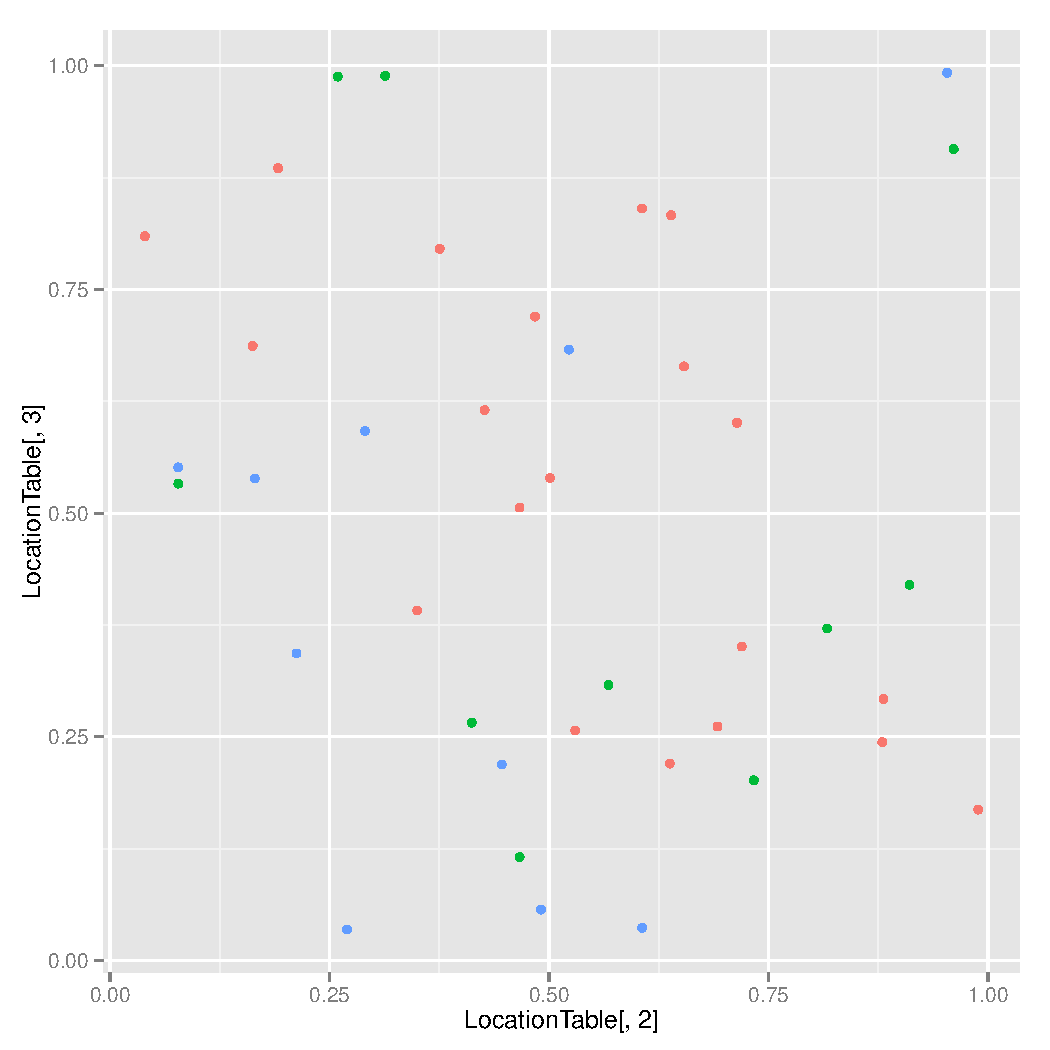
\includegraphics[width=\maxwidth]{figure/unnamed-chunk-2-1} 
\begin{kframe}\begin{verbatim}
##   Count                           Happy Testpool Threshold
## R     1  1 0.88087670 0.292274361     0        5         2
## R     2  1 0.50111460 0.539329507     0        5         2
## R     3  1 0.34984375 0.391174800     0        5         2
## R     4  1 0.71935381 0.350873383     0        5         2
## R     5  1 0.46636470 0.506259974     0        5         2
## R     6  1 0.37548038 0.795474492     0        5         2
## R     7  1 0.48403496 0.719710088     0        5         2
## R     8  1 0.16247257 0.686906370     0        5         2
## R     9  1 0.19127365 0.885605896     0        5         2
## R    10  1 0.71405276 0.600972072     0        5         2
## R    11  1 0.60577097 0.840487010     0        5         2
## R    12  1 0.63742605 0.220050183     0        5         2
## R    13  1 0.03969718 0.809529376     0        5         2
## R    14  1 0.69181073 0.261534572     0        5         2
## R    15  1 0.65363839 0.664152477     0        5         2
## R    16  1 0.63901260 0.833021256     0        5         2
## R    17  1 0.52979992 0.257004289     0        5         2
## R    18  1 0.98889149 0.168652831     0        5         2
## R    19  1 0.42661108 0.615167781     0        5         2
## R    20  1 0.87949560 0.244099568     0        5         2
## R    21  1 0.31329813 0.988823090     0        5         2
## R    22  1 0.41195102 0.265774416     0        5         2
## R    23  1 0.25931412 0.987915983     0        5         2
## R    24  1 0.73325532 0.201447914     0        5         2
## R    25  1 0.07781230 0.533021456     0        5         2
## R    26  1 0.96087329 0.906998900     0        5         2
## R    27  1 0.56762140 0.308037600     0        5         2
## R    28  1 0.81676286 0.371100862     0        5         2
## R    29  1 0.46643300 0.115485445     0        5         2
## R    30  1 0.91045513 0.420044321     0        5         2
## R    31  1 0.95330606 0.992173342     0        5         2
## R    32  1 0.21233086 0.343192349     0        5         2
## R    33  1 0.60603245 0.036496113     0        5         2
## R    34  1 0.49077000 0.056881471     0        5         2
## R    35  1 0.07772721 0.551119528     0        5         2
## R    36  1 0.52250407 0.682729156     0        5         2
## R    37  1 0.44620386 0.219016305     0        5         2
## R    38  1 0.26996361 0.034623944     0        5         2
## R    39  1 0.16472249 0.538759632     0        5         2
## R    40  1 0.29034521 0.591719521     0        5         2
## R    41  1 0.36602488 0.506071298     0        5         2
## R    42  1 0.95998975 0.430965685     0        5         2
## R    43  1 0.18552025 0.682198081     0        5         2
## R    44  1 0.29617673 0.260350465     0        5         2
## R    45  1 0.08887899 0.881948053     0        5         2
## R    46  1 0.14174181 0.801370089     0        5         2
## R    47  1 0.32205100 0.806377763     0        5         2
## R    48  1 0.68550996 0.519523249     0        5         2
## R    49  1 0.39148476 0.910894458     0        5         2
## R    50  1 0.90343921 0.725260953     0        5         2
## G    51  0 0.38196612 0.288304984     0        5         2
## G    52  0 0.60736101 0.437951637     0        5         2
## G    53  0 0.28304754 0.553282319     0        5         2
## G    54  0 0.95431985 0.335656283     0        5         2
## G    55  0 0.76918250 0.062349494     0        5         2
## G    56  0 0.70062206 0.985571126     0        5         2
## G    57  0 0.90407563 0.291436276     0        5         2
## G    58  0 0.97487034 0.866844861     0        5         2
## G    59  0 0.57538006 0.747099884     0        5         2
## G    60  0 0.56372344 0.376455617     0        5         2
## G    61  0 0.51646822 0.596139638     0        5         2
## G    62  0 0.25671389 0.175912370     0        5         2
## G    63  0 0.85005458 0.500281350     0        5         2
## G    64  0 0.52127557 0.191887318     0        5         2
## G    65  0 0.99933825 0.186784270     0        5         2
## G    66  0 0.90205565 0.310173962     0        5         2
## G    67  0 0.11732077 0.693351585     0        5         2
## G    68  0 0.15488647 0.189495955     0        5         2
## G    69  0 0.90067305 0.316219866     0        5         2
## G    70  0 0.45880769 0.064337363     0        5         2
## G    71  0 0.92430297 0.083698585     0        5         2
## G    72  0 0.41358364 0.518244113     0        5         2
## G    73  0 0.81491619 0.366424271     0        5         2
## G    74  0 0.89288318 0.669900519     0        5         2
## G    75  0 0.83698380 0.592185493     0        5         2
## G    76  0 0.91252799 0.971544161     0        5         2
## G    77  0 0.49615943 0.124587787     0        5         2
## G    78  0 0.06626001 0.932025275     0        5         2
## G    79  0 0.19143956 0.454173630     0        5         2
## G    80  0 0.12666432 0.033178403     0        5         2
## G    81  0 0.55324639 0.159727750     0        5         2
## G    82  0 0.69469408 0.928274332     0        5         2
## G    83  0 0.60196479 0.674556291     0        5         2
## G    84  0 0.55610809 0.095542465     0        5         2
## G    85  0 0.17690371 0.500974125     0        5         2
## G    86  0 0.58767244 0.235076410     0        5         2
## G    87  0 0.57664420 0.595454185     0        5         2
## G    88  0 0.25248506 0.373429720     0        5         2
## G    89  0 0.80710407 0.954102898     0        5         2
## G    90  0 0.11780056 0.845909939     0        5         2
## G    91  0 0.03558219 0.340554802     0        5         2
## G    92  0 0.92623339 0.010365395     0        5         2
## G    93  0 0.00783140 0.643187550     0        5         2
## G    94  0 0.48946651 0.190491560     0        5         2
## G    95  0 0.26242574 0.907880367     0        5         2
## G    96  0 0.61903045 0.817983840     0        5         2
## G    97  0 0.04407600 0.533258923     0        5         2
## G    98  0 0.65611025 0.014729884     0        5         2
## G    99  0 0.99759068 0.708671428     0        5         2
## G   100  0 0.70825015 0.855745154     0        5         2
## B   101 -1 0.28403739 0.682381599     0        5         2
## B   102 -1 0.49549380 0.317354294     0        5         2
## B   103 -1 0.01665007 0.856748833     0        5         2
## B   104 -1 0.36686837 0.644468423     0        5         2
## B   105 -1 0.15136172 0.909936710     0        5         2
## B   106 -1 0.99574788 0.274148161     0        5         2
## B   107 -1 0.34591864 0.068874221     0        5         2
## B   108 -1 0.73146704 0.714227306     0        5         2
## B   109 -1 0.86064525 0.210119003     0        5         2
## B   110 -1 0.96896713 0.616654244     0        5         2
## B   111 -1 0.37609992 0.134423233     0        5         2
## B   112 -1 0.53699035 0.988473766     0        5         2
## B   113 -1 0.26198562 0.431435353     0        5         2
## B   114 -1 0.44866089 0.609484812     0        5         2
## B   115 -1 0.61410004 0.489205373     0        5         2
## B   116 -1 0.48478954 0.284334196     0        5         2
## B   117 -1 0.54874250 0.059020051     0        5         2
## B   118 -1 0.12959936 0.537379685     0        5         2
## B   119 -1 0.01384381 0.788933858     0        5         2
## B   120 -1 0.14618622 0.523666771     0        5         2
## B   121 -1 0.88337735 0.862787974     0        5         2
## B   122 -1 0.26621716 0.459968218     0        5         2
## B   123 -1 0.44061894 0.570699342     0        5         2
## B   124 -1 0.77261437 0.497840131     0        5         2
## B   125 -1 0.27200541 0.029366484     0        5         2
## B   126 -1 0.34462786 0.651964305     0        5         2
## B   127 -1 0.42271211 0.566269456     0        5         2
## B   128 -1 0.11508901 0.602072069     0        5         2
## B   129 -1 0.30451388 0.993687095     0        5         2
## B   130 -1 0.16626382 0.570786456     0        5         2
## B   131 -1 0.29007546 0.607338065     0        5         2
## B   132 -1 0.37406760 0.154123175     0        5         2
## B   133 -1 0.50591913 0.375157764     0        5         2
## B   134 -1 0.18329200 0.622406428     0        5         2
## B   135 -1 0.12450300 0.448399968     0        5         2
## B   136 -1 0.99320260 0.935470444     0        5         2
## B   137 -1 0.90531437 0.085126241     0        5         2
## B   138 -1 0.10787591 0.051739027     0        5         2
## B   139 -1 0.31719869 0.540758874     0        5         2
## B   140 -1 0.74466186 0.145718680     0        5         2
## B   141 -1 0.95939913 0.009733661     0        5         2
## B   142 -1 0.98383691 0.508911631     0        5         2
## B   143 -1 0.19343030 0.248508668     0        5         2
## B   144 -1 0.02300792 0.544214905     0        5         2
## B   145 -1 0.05023313 0.631581234     0        5         2
## B   146 -1 0.18296334 0.046411481     0        5         2
## B   147 -1 0.29731931 0.511776394     0        5         2
## B   148 -1 0.72596524 0.908810235     0        5         2
## B   149 -1 0.66749887 0.074263743     0        5         2
## B   150 -1 0.63282073 0.183889588     0        5         2
##        [,1] [,2] [,3] [,4] [,5]
##   [1,]   57   66   69   20  109
##   [2,]    5   61  123  127  114
##   [3,]  113   88   51  122   41
##   [4,]   14   73   28   52   24
##   [5,]    2   72  123  127   41
##   [6,]   47   49    7  101  126
##   [7,]   36   59  114   19   83
##   [8,]   43   67  134  128  130
##   [9,]  105   95   90   46   45
##  [10,]   48   15  108  124   75
##  [11,]   96   16   59  100   82
##  [12,]  150   86   14   24   81
##  [13,]  119  103   90   45   46
##  [14,]   12   24    4  150   86
##  [15,]   83   10  108   87   59
##  [16,]   96   11  100   59   82
##  [17,]  116   86   27   64  102
##  [18,]   65  106   71  137   20
##  [19,]  114  123  127  104  126
##  [20,]  109    1   57   66   69
##  [21,]  129   23   95   49    9
##  [22,]   51   37  116  102   94
##  [23,]  129   21   95    9  105
##  [24,]  140   14   12  150  109
##  [25,]   35   97  118  144  120
##  [26,]   58  136   76   31  121
##  [27,]   17   60  102   86  116
##  [28,]   73    4   69    1   66
##  [29,]   77   70   34   94   84
##  [30,]   42   54   63   69   28
##  [31,]   76  136   26   58  121
##  [32,]   88  143  113   79   44
##  [33,]   98  117  149   84   34
##  [34,]   70  117   29   77   84
##  [35,]   25   97  118  144  128
##  [36,]    7   83   59   61   87
##  [37,]   94   22  116   64   17
##  [38,]  125  107  146   62   80
##  [39,]  120  130  118   85  128
##  [40,]  131   53  139  147  126
##  [41,]   72  139  147  127   53
##  [42,]   30  142   54   69   63
##  [43,]    8  134   67  101  128
##  [44,]   51   62  143   22   32
##  [45,]   90   78  105  103   13
##  [46,]   90   45    9   13  105
##  [47,]    6   95   49  101    9
##  [48,]  115   10  124   52   87
##  [49,]   21    6  129   47   95
##  [50,]   74   99  110  121   75
##  [51,]   22   44   37  116    3
##  [52,]  115   60   48  133   27
##  [53,]  139   40  147  131  122
##  [54,]   69   66   57  106    1
##  [55,]  140  149   98  137   24
##  [56,]   82  148   89  100  112
##  [57,]   66    1   69   20   54
##  [58,]   26  136  121   76   31
##  [59,]   83   96   36    7   11
##  [60,]  133   27   52  102  116
##  [61,]    2   87  114  123   36
##  [62,]   44  143   68  132  111
##  [63,]  124   75   30   42   28
##  [64,]   94   81   17   77   86
##  [65,]   18  106   71   20  137
##  [66,]   69   57    1   54   20
##  [67,]    8   43  145  128  134
##  [68,]  143   62  138  146   44
##  [69,]   66   57    1   54   20
##  [70,]   34   29   77  117   84
##  [71,]  137   92  141   18   65
##  [72,]  127   41    5  123    2
##  [73,]   28    4    1   69   66
##  [74,]   50  110   75   99  108
##  [75,]   63   74  124   10  110
##  [76,]   31   26  136   89  121
##  [77,]   29   94   84   81   34
##  [78,]   45  105  103   90   13
##  [79,]   85  135  113  122  120
##  [80,]  138  146   38  125   68
##  [81,]   64   84   77   94   86
##  [82,]  148   56  100   16   89
##  [83,]   15   59   36   87   61
##  [84,]  117   81   77   34   33
##  [85,]  120   39   79  118  130
##  [86,]   12   17  150   27   64
##  [87,]   61   83    2   36   15
##  [88,]   32  113  122    3   79
##  [89,]  148   76   56   82  121
##  [90,]   45   46  105    9   13
##  [91,]  135   32  143   68   79
##  [92,]  141   71  137   55   18
##  [93,]  145  144  128   35   97
##  [94,]   64   37   77   81   17
##  [95,]    9   23  129   21  105
##  [96,]   16   11   59  100   82
##  [97,]  144   25   35  118  145
##  [98,]   33  149  117   55   84
##  [99,]   50  110   74   58  121
## [100,]  148   16   82   96   11
## [101,]  126  131   40  104   43
## [102,]  116  133   17   27   60
## [103,]   13  119   45   78   90
## [104,]  126   19  131  114  101
## [105,]    9   45   90   78   46
## [106,]   54   65   57   66   69
## [107,]  111   38  125  132   70
## [108,]   15   10   83  100   16
## [109,]   20    1   57   66   69
## [110,]   74   99  142   50   75
## [111,]  132  107   29   70   37
## [112,]   11   56   49   82   16
## [113,]  122   88   79  147    3
## [114,]   19  123  127   61    2
## [115,]   52   48   87   60    2
## [116,]  102   17   22   37   27
## [117,]   84   34   33   77   70
## [118,]  120   39  130   25   35
## [119,]   13  103   90   45   46
## [120,]  118   39   85  130   25
## [121,]   26   58   76   89  136
## [122,]  113  147   79   88   53
## [123,]  127  114   19   72    2
## [124,]   63   48   75   10   28
## [125,]   38  107  146   80   62
## [126,]  104  101  131   40   19
## [127,]  123   72   19  114    5
## [128,]  130   35  118  134  145
## [129,]   21   23   95   49    9
## [130,]   39  118  120  134  128
## [131,]   40   53  126  139  101
## [132,]  111  107   37   29   22
## [133,]   60  102   27  116   52
## [134,]  130   43    8  128   39
## [135,]   79   85  120  118   25
## [136,]   26   31   58   76  121
## [137,]   71   92  141   18  109
## [138,]   80  146   68   38  125
## [139,]  147   53   40   41  131
## [140,]   24   55  149  150   14
## [141,]   92   71  137   18   65
## [142,]   42  110   30   63   75
## [143,]   68   62   32   44   88
## [144,]   97   35   25  145   93
## [145,]   93  128   35   67  144
## [146,]   80  138   38  125   68
## [147,]  139   53  122   41   40
## [148,]   82  100   56   89   16
## [149,]   98   33   55  140   84
## [150,]   12   86   81   14   24
\end{verbatim}
\end{kframe}
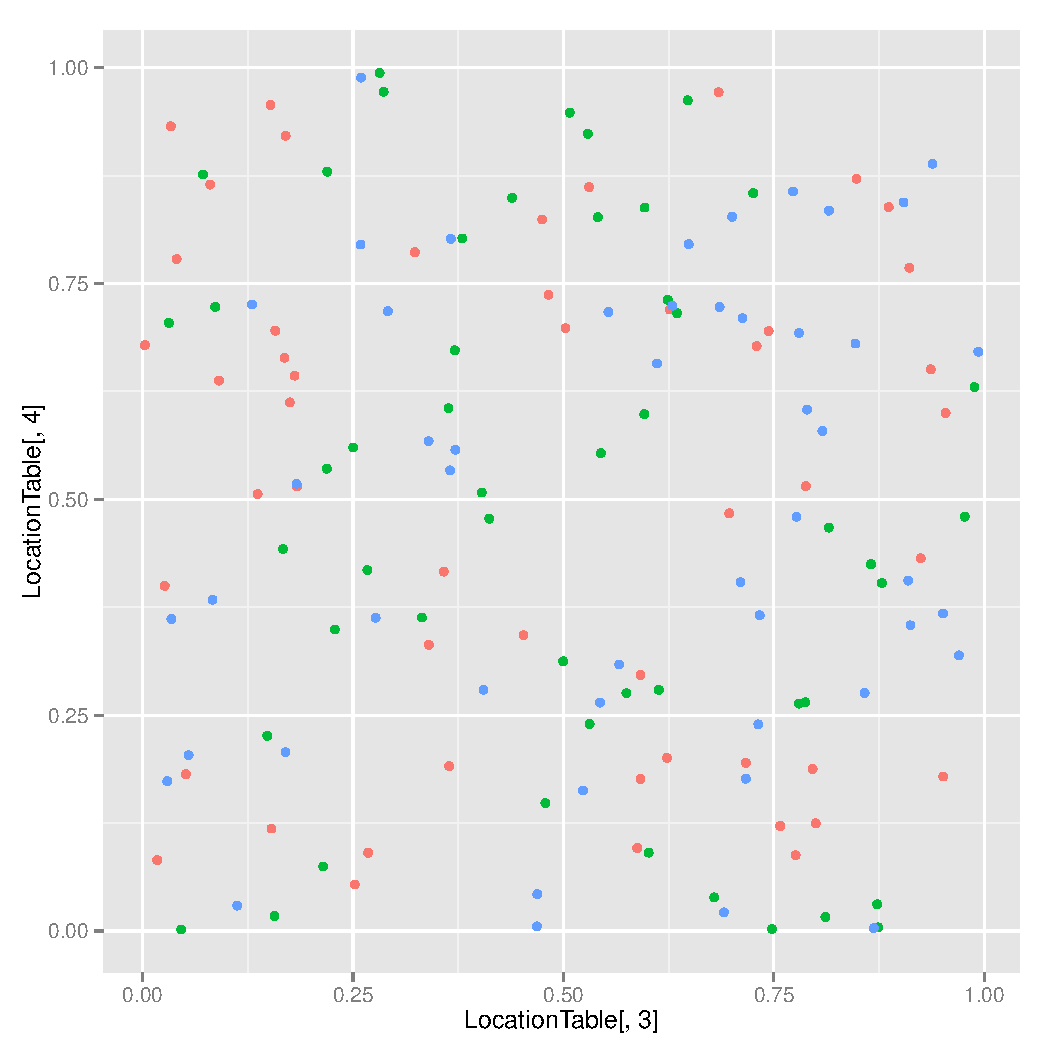
\includegraphics[width=\maxwidth]{figure/unnamed-chunk-2-2} 
\begin{kframe}\begin{verbatim}
## [1]   8 143
\end{verbatim}
\begin{alltt}
\hlcom{# print(system.time(Schelling(testRacialPreferenceTable)))}
\end{alltt}
\end{kframe}
\end{knitrout}

\section{Code Review}
\subsection{Sketch model that code is based  on}





\end{document}
